%%% Hlavní soubor. Zde se definují základní parametry a odkazuje se na ostatní části. %%%

%% Verze pro jednostranný tisk:
% Okraje: levý 40mm, pravý 25mm, horní a dolní 25mm
% (ale pozor, LaTeX si sám přidává 1in)
\documentclass[12pt,a4paper]{report}
\setlength\textwidth{145mm}
\setlength\textheight{247mm}
\setlength\oddsidemargin{15mm}
\setlength\evensidemargin{15mm}
\setlength\topmargin{0mm}
\setlength\headsep{0mm}
\setlength\headheight{0mm}
% \openright zařídí, aby následující text začínal na pravé straně knihy
\let\openright=\clearpage

%% Pokud tiskneme oboustranně:
% \documentclass[12pt,a4paper,twoside,openright]{report}
% \setlength\textwidth{145mm}
% \setlength\textheight{247mm}
% \setlength\oddsidemargin{15mm}
% \setlength\evensidemargin{0mm}
% \setlength\topmargin{0mm}
% \setlength\headsep{0mm}
% \setlength\headheight{0mm}
% \let\openright=\cleardoublepage

%% Použité kódování znaků: obvykle latin2, cp1250 nebo utf8:
\usepackage[utf8]{inputenc}

%% Ostatní balíčky
\usepackage{graphicx}
\usepackage{amsthm}

%% Balíček hyperref, kterým jdou vyrábět klikací odkazy v PDF,
%% ale hlavně ho používáme k uložení metadat do PDF (včetně obsahu).
%% POZOR, nezapomeňte vyplnit jméno práce a autora.
\usepackage[unicode]{hyperref}   % Musí být za všemi ostatními balíčky
\hypersetup{pdftitle=Název práce}
\hypersetup{pdfauthor=Jméno Příjmení}

%%% Drobné úpravy stylu

% Tato makra přesvědčují mírně ošklivým trikem LaTeX, aby hlavičky kapitol
% sázel příčetněji a nevynechával nad nimi spoustu místa. Směle ignorujte.
\makeatletter
\def\@makechapterhead#1{
  {\parindent \z@ \raggedright \normalfont
   \Huge\bfseries \thechapter. #1
   \par\nobreak
   \vskip 20\p@
}}
\def\@makeschapterhead#1{
  {\parindent \z@ \raggedright \normalfont
   \Huge\bfseries #1
   \par\nobreak
   \vskip 20\p@
}}
\makeatother

% Toto makro definuje kapitolu, která není očíslovaná, ale je uvedena v obsahu.
\def\chapwithtoc#1{
\chapter*{#1}
\addcontentsline{toc}{chapter}{#1}
}

\begin{document}

% Trochu volnější nastavení dělení slov, než je default.
\lefthyphenmin=2
\righthyphenmin=2

%%% Titulní strana práce

\pagestyle{empty}
\begin{center}

\large

Charles University in Prague

\medskip

Faculty of Mathematics and Physics

\vfill

{\bf\Large MASTER THESIS}

\vfill

\centerline{\mbox{
\includegraphics[width=60mm]{img/logo.pdf}}}

\vfill
\vspace{5mm}

{\LARGE First and last name of the author}

\vspace{15mm}

% Název práce přesně podle zadání
{\LARGE\bfseries Title of the thesis}

\vfill

% Název katedry nebo ústavu, kde byla práce oficiálně zadána
% (dle Organizační struktury MFF UK)
Name of the department or institute

\vfill

\begin{tabular}{rl}

Supervisor of the master thesis: & First and last name \\
\noalign{\vspace{2mm}}
Study programme: & programme \\
\noalign{\vspace{2mm}}
Specialization: & specialization \\
\end{tabular}

\vfill

% Zde doplňte rok
Prague YEAR

\end{center}

\newpage

%%% Následuje vevázaný list -- kopie podepsaného "Zadání diplomové práce".
%%% Toto zadání NENÍ součástí elektronické verze práce, nescanovat.

%%% Na tomto místě mohou být napsána případná poděkování (vedoucímu práce,
%%% konzultantovi, tomu, kdo zapůjčil software, literaturu apod.)

\openright

\noindent
Dedication.

\newpage

%%% Strana s čestným prohlášením k diplomové práci

\vglue 0pt plus 1fill

\noindent
I declare that I carried out this master thesis independently, and only with the cited
sources, literature and other professional sources.

\medskip\noindent
I understand that my work relates to the rights and obligations under the Act No.
121/2000 Coll., the Copyright Act, as amended, in particular the fact that the Charles
University in Prague has the right to conclude a license agreement on the use of this
work as a school work pursuant to Section 60 paragraph 1 of the Copyright Act.

\vspace{10mm}

\hbox{\hbox to 0.5\hsize{%
In ........ date ............
\hss}\hbox to 0.5\hsize{%
signature of the author
\hss}}

\vspace{20mm}
\newpage

%%% Povinná informační strana diplomové práce

\vbox to 0.5\vsize{
\setlength\parindent{0mm}
\setlength\parskip{5mm}

Název práce:
Název práce
% přesně dle zadání

Autor:
Jméno a příjmení autora

Katedra:  % Případně Ústav:
Název katedry či ústavu, kde byla práce oficiálně zadána
% dle Organizační struktury MFF UK

Vedoucí diplomové práce:
Jméno a příjmení s tituly, pracoviště
% dle Organizační struktury MFF UK, případně plný název pracoviště mimo MFF UK

Abstrakt:
% abstrakt v rozsahu 80-200 slov; nejedná se však o opis zadání diplomové práce

Klíčová slova:
% 3 až 5 klíčových slov

\vss}\nobreak\vbox to 0.49\vsize{
\setlength\parindent{0mm}
\setlength\parskip{5mm}

Title:
% přesný překlad názvu práce v angličtině

Author:
Jméno a příjmení autora

Department:
Název katedry či ústavu, kde byla práce oficiálně zadána
% dle Organizační struktury MFF UK v angličtině

Supervisor:
Jméno a příjmení s tituly, pracoviště
% dle Organizační struktury MFF UK, případně plný název pracoviště
% mimo MFF UK v angličtině

Abstract:
% abstrakt v rozsahu 80-200 slov v angličtině; nejedná se však o překlad
% zadání diplomové práce

Keywords:
% 3 až 5 klíčových slov v angličtině

\vss}

\newpage

%%% Strana s automaticky generovaným obsahem diplomové práce. U matematických
%%% prací je přípustné, aby seznam tabulek a zkratek, existují-li, byl umístěn
%%% na začátku práce, místo na jejím konci.

\openright
\pagestyle{plain}
\setcounter{page}{1}
\tableofcontents

%%% Jednotlivé kapitoly práce jsou pro přehlednost uloženy v samostatných souborech
\chapter{Introduction}
\addcontentsline{toc}{chapter}{Introduction}
Today's processors have multiple cores and it's single core performance is improving only very slow because of physical limitations. On the other hand number of cores is still increasing and we can assume that it will continue. That's why developing parallel software is crucial for improving overall performance.

Parallelization can be achieved manually or using some framework designed for it. For example there are frameworks like OpenMP or Intel TBB. Department of Software Engineering at Charles University in Prague developed it's own parallelization framework called Bobox\cite{bobox}.

Bobox is designed for parallel processing large amounts of data. It was specifically created to simplify and speed up parallel programming of certain class of problems - data computations based on non-linear pipeline. It was successfully used in implementation of XQuery and TriQuery engines.

Bobox consists from runtime environment and operators. These operators are called boxes and they are C++ implementation of data processing algorithms. Boxes use messages called envelopes to send processed data to each other. 

Bobox takes as input execution plan written in special language Bobolang\cite{bobolang}. It allows to define used boxes and simply connect then into directed acyclic graph. Bobolang specifies the structure of whole application. It can create highly optimized evaluation, which is capable of using the most of the hardware resources.

Most used databases are relational. They are based on the view of data organized in tables called relations. SQL\cite{database} ("Structured query language") is very important language based on relational databases. It is used for querying data, modifying content of tables and also the structure of tables.

Architecture of planned SQL compiler is displayed in figure~\ref{fig:sqlarchitecture}. 
\begin{figure}[h!]
  \centering

    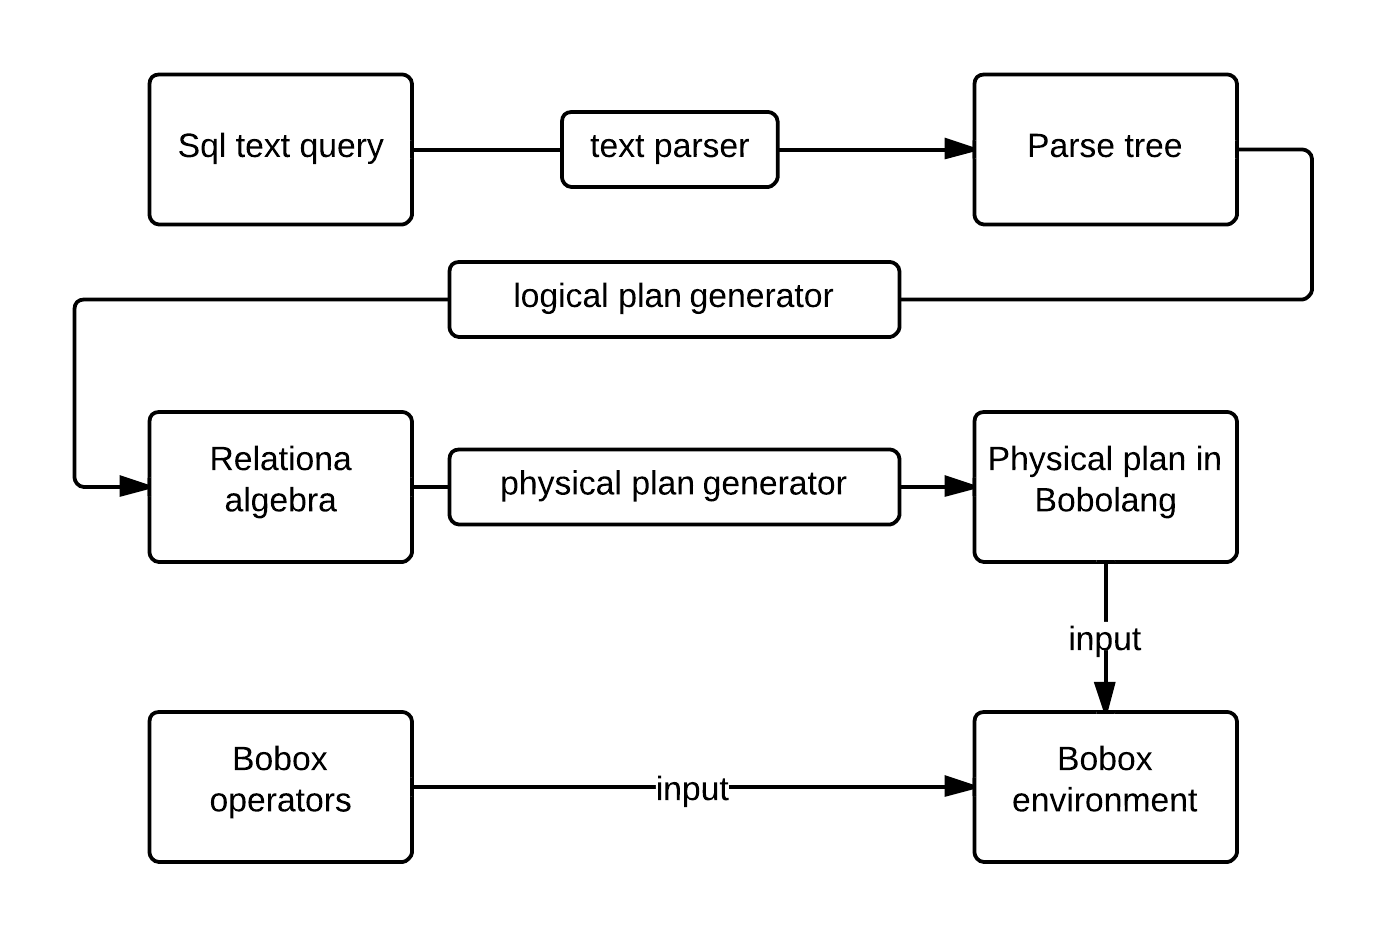
\includegraphics[width=1\textwidth]{sqlarchitecture}
    
      \caption{SQL compiler architecture.}
        \label{fig:sqlarchitecture}
\end{figure}
SQL query is written in text. This text is parsed into parse tree, which is transformed into logical query plan (Relational algebra). Relational algebra is then optimized and this form is used for generating physical query plan. Physical plan written in Bobolang is input for Bobox for execution. Physical plan is not enough, we need to provide implementation of physical algorithms (Bobox operators).

Since SQL is a pretty complicated language, this thesis aim is only implementing optimization and transformation of logical plan into physical plan. This part is displayed as physical plan generator in figure~\ref{fig:sqlarchitecture}.


The main goal of this thesis is to implement part of SQL compiler. The input is query written in XML format in from of relational algebra. Program reads input and builds relational algebra tree, which is then checked for semantic errors. Then we improve logical plan by pushing selection down the tree. From improved relational algebra tree we generate physical plan. In this phase we assign physical algorithm for every logical plan operator and we also choose order of joins. The output is execution plan for Bobox written in Bobolang.

\chapter{Architecture}

\section{Bobox}

In the section we describe basic architecture of Bobox. Information source for this chapter is Doctoral thesis\cite{faltthesis}. 

Overall Bobox architecture is displayed in figure~\ref{fig:bobox}. Framework contains of Boxes. Box is basically a C++ class containing implementation of data processing algorithm or it can be set of connected boxes. Box can have arbitrary number of inputs and outputs. All boxes are connected to a directed acyclic graph.  

\begin{figure}[h!]
  \centering
    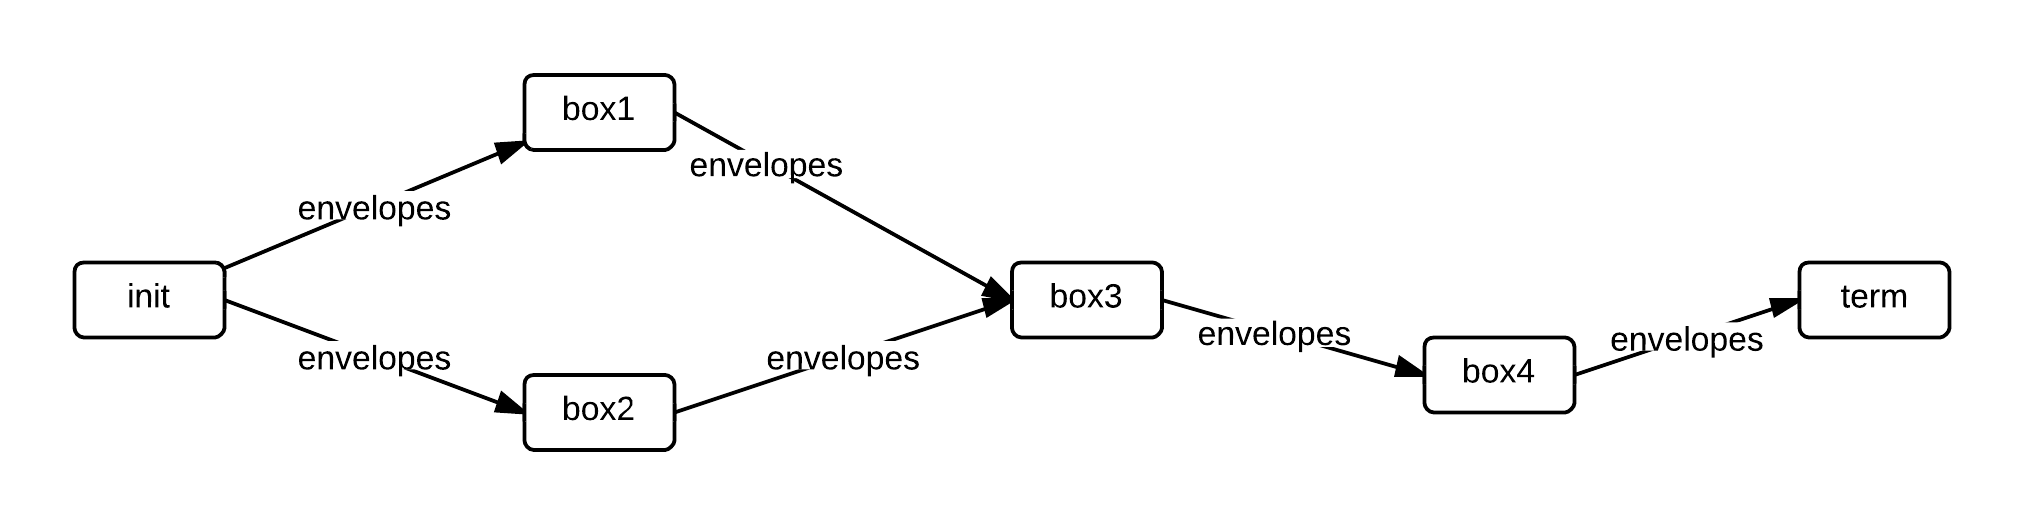
\includegraphics[width=1\textwidth]{bobox}

      \caption{Bobox architecture.}
          \label{fig:bobox}
\end{figure}

Data streams are implemented as streams of data units called envelopes. Envelope structure is displayed in figure~\ref{fig:envelope}. It consists of sequence tuples, but internally data are stored by columns, that means envelope contains from sequence of columns and it's data is stored in separate list. So to read all attributes of the i-th tuple we have to access all column lists and read it's i-th element. There is special type of envelope having poisoned pill. It is send after all valid data indicating end of data stream. 

\begin{figure}[h!]
  \centering
    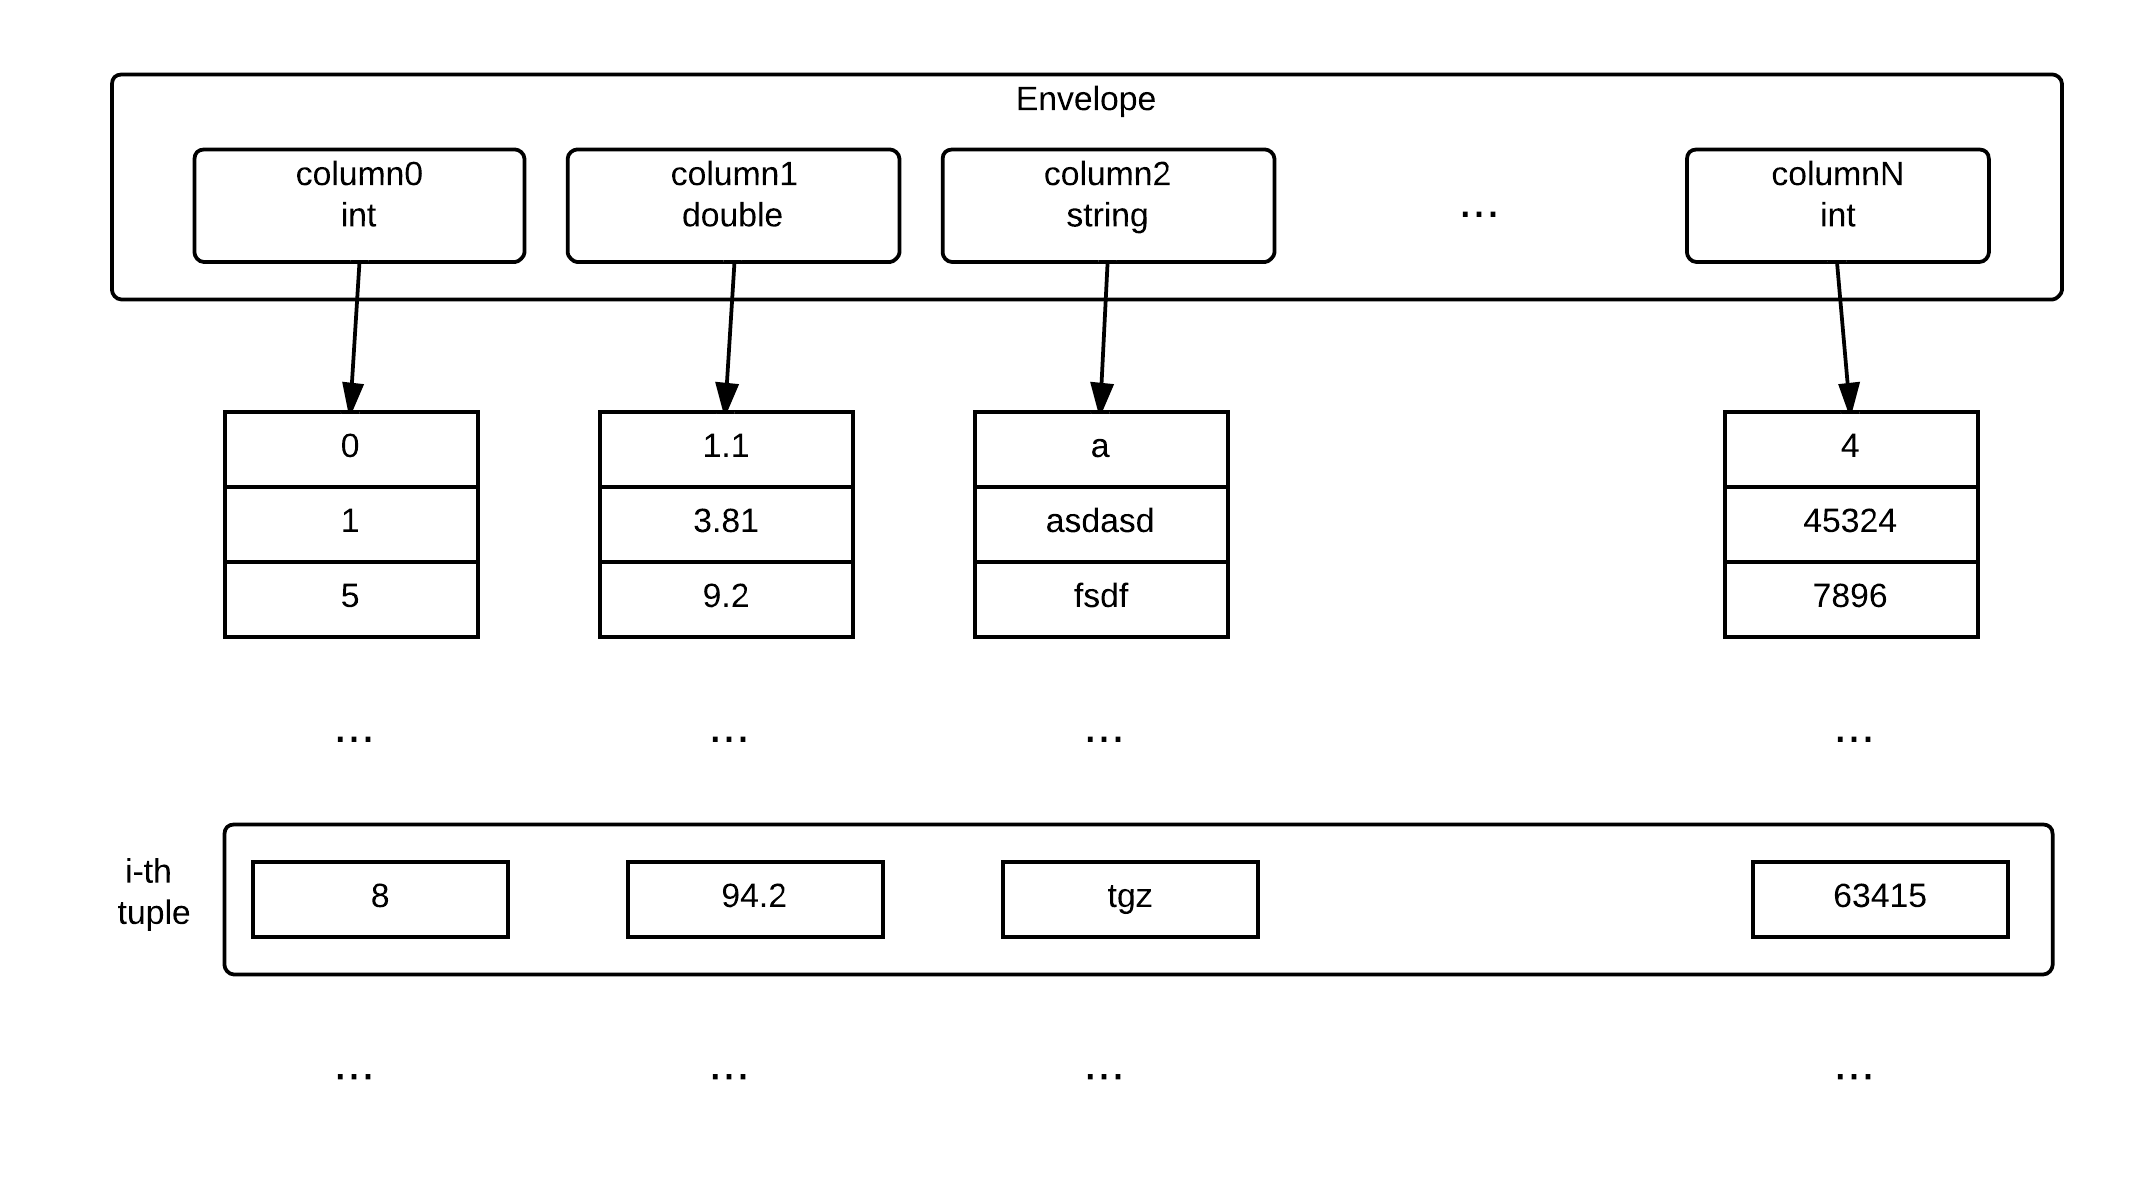
\includegraphics[width=1\textwidth]{envelope}

      \caption{Envelope structure.}
          \label{fig:envelope}
\end{figure}
There are two special boxes, which have to be in every execution plan:
\begin{itemize}


\item $init$ - first box in topological order and it indicates starting box of execution plan

\item $term$ - last box in topological order and indicates that plan has been completely evaluated

\end{itemize}

Evaluation starts with scheduling $init$ box, which sends poisoned pills to all of its output. All of it's output boxes will be scheduled. They can read data from hard drive or network, process it and sent it to other boxes for further processing. Other boxes usually receives data in envelopes in their inputs. Box $term$ waits for every it's input to receive poisoned pill and then evaluation ends.

\section{Bobolang}
In this section we describe syntax and semantics of Bololang language. We used paper\cite{bobolang} as information source.

Bobolang is a formal description language for Bobox execution plan. Bobox environment provides implementation of basic operators (boxes). Bobolang let's programmer choose which boxes to used, what boxes to use, what type are passed and how the boxes are interconnected. 

We can define whole execution plan using operator main with empty input and output. Example of whole Bobolang plan:

\begin{verbatim}
operator main()->()
{
    source()->(int) src;
    process(int)->(int,int,int) proc;
    sink(int,int,int)->() sink;

    input -> src -> proc; 
    proc -> sink;
    sink -> output;
}
\end{verbatim}

In the first part we declare operators, define type of input and output. For every declared operator we provide identifier. Second part specifies connection between declared operators. Code \verb|op1 -> op2| indicates that output of \verb|op1| is connected to input of operator \verb|op2|. In this case output type of \verb|op1| has equal to input type of \verb|op2|. Bobolang syntax also allows to create chains of operators like \verb|op1 -> op3| which has semantics like \verb|op1 -> op2| and \verb|op2 -> op3|. 

There are explicitly defined operators called \verb|input| and \verb|output|. They represents input and output of declared operator \verb|process|. The line \verb|input -> srce;| represents that input of the operator \verb|process| is connected to output of operator \verb|pre|.

Boblang also allows to declare operators with empty input or output. They have type \verb|()| that means it doesn't transfer any data. Only data allowed is to transfer poisoned pill. When box receives poisoned pill, it means that it should start working, Sending it means that it's work is done.


 In figure~\ref{fig:exampleplan} we can seen structure of example execution plan. Operators \verb|init| and \verb|term| are added automatically. Operator \verb|init| sends poisoned pill to \verb|source|, which can read data from hard drive or network. These data are send to box \verb|process|. Operator sink stores data and sends poisoned pill to box \verb|term| and the computation ends.
\begin{figure}[h!]
  \centering

    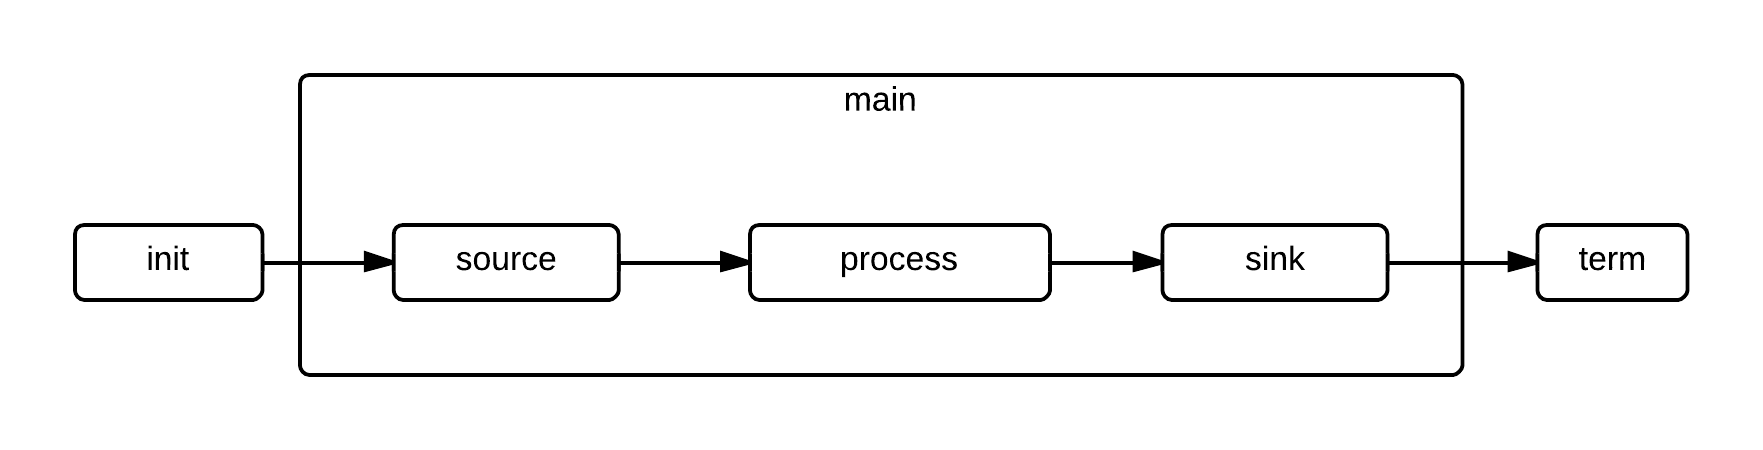
\includegraphics[width=1\textwidth]{exampleplan}
    
      \caption{Example of execution plan.}
        \label{fig:exampleplan}
\end{figure}





\chapter{Title of the second chapter}

\section{Title of the first subchapter of the second chapter}

\section{Title of the second subchapter of the second chapter}


% Ukázka použití některých konstrukcí LateXu (odkomentujte, chcete-li)
% %%% Ukázka použití některých konstrukcí LaTeXu

\subsection{Ukázka \LaTeX{}u}
\label{ssec:ukazka}

This short subsection serves as an~example of basic \LaTeX{} constructs,
which can be useful for writing a~thesis.

Let us start with lists:

\begin{itemize}
\item The logo of Matfyz is displayed in figure~\ref{fig:mff}.
\item This is subsection~\ref{ssec:ukazka}.
\item Citing literature~\cite{lamport94}.
\end{itemize}

Different kinds of dashes:
red-black (short),
pages 16--22 (middle),
$45-44$ (minus),
and this is --- as you could have expected --- a~sentence-level dash,
which is the longest.
(Note that we have follwed \verb|a| by a~tilde instead of a~space
to avoid line breaks at that place.)

\newtheorem{theorem}{Theorem}
\newtheorem*{define}{Definition}	% Definice nečíslujeme, proto "*"

\begin{define}
A~{\sl Tree} is a connected graph with no cycles.
\end{define}

\begin{theorem}
This theorem is false.
\end{theorem}

\begin{proof}
False theorems do not have proofs.
\end{proof}

\begin{figure}
	\centering
	
\includegraphics[width=30mm]{../img/logo.eps}
	\caption{Logo of MFF UK}
	\label{fig:mff}
\end{figure}


\chapter{Conclusion}
\addcontentsline{toc}{chapter}{Conclusion}

The aim of this thesis was to implement part of the SQL compiler. Created program reads input relational algebra, optimizes it and generated physical plan from it. Output is written in Bobolang.

After the introduction we described Bobox and Bobolang. Next chapter contains theory used to implement query transformer. Chapter analysis contains description of used algorithms and important data structures used in implemented tool. Final chapter describe some implementation details of created program.

Created software is a first tool of planed SQL compiler. Front end, which transforms text query to relational algebra, is not yet implemented. At the time of submitting this thesis, the all Bobox runtime operators are not implemented. That's why we couldn't evaluate any queries to prove that plans are correct.

We tested software by transforming some simple queries and queries from benchmark\cite{benchmark}. We can only check generated plans by looking generated debug outputs. From the results we can say that generated plans look correct and also optimal. Based on this result we can say, that this thesis fulfilled it's aim. 


Implemented tool can be improved by adding more logical plan optimizations. We can add also support for more algorithms like nested loop joins.



%%% Seznam použité literatury
%%% Seznam použité literatury je zpracován podle platných standardů. Povinnou citační
%%% normou pro diplomovou práci je ISO 690. Jména časopisů lze uvádět zkráceně, ale jen
%%% v kodifikované podobě. Všechny použité zdroje a prameny musí být řádně citovány.

\def\bibname{Bibliography}
\begin{thebibliography}{99}
\addcontentsline{toc}{chapter}{\bibname}

\bibitem{bobox}
  D. Bednárek, J. Dokulil, J. Yaghob, and F. Zavoral.
  \emph{Bobox: Parallelization
  framework for data processing. Advances in Information Technology and
  Applied Computing}, 2012.
  
\bibitem{bobolang}
   Z. Falt, , D. Bednárek, K. Martin, J. Yaghob, and F. Zavoral.
  \emph{Bobolang - a language for parallel streaming applications.}  In 23rd international sym-
      posium on High-Performance Parallel and Distributed Computing. ACM,
      2014.
  
\bibitem{database}
   H. Garcia-Molina, J. D. Ullman, J. Widom.
  \emph{Database Systems The Complete Book}. Prentice Hall, 2002,
 ISBN 0-13-031995-3.

\bibitem{faltthesis}
  Zbyněk Falt.
  \emph{Parallel Processing of Data - Doctoral thesis}. Prague, 2013.

\bibitem{benchmark}
 \emph{ TPC BENCHMARK TM H},
 Standard Specification, Revision 2.15.0

\bibitem{xerces}
 \emph{ Xerces-C++},
http://xerces.apache.org/xerces-c/

\end{thebibliography}


%%% Tabulky v diplomové práci, existují-li.
\chapwithtoc{List of Tables}

%%% Použité zkratky v diplomové práci, existují-li, včetně jejich vysvětlení.
\chapwithtoc{List of Abbreviations}

%%% Přílohy k diplomové práci, existují-li (různé dodatky jako výpisy programů,
%%% diagramy apod.). Každá příloha musí být alespoň jednou odkazována z vlastního
%%% textu práce. Přílohy se číslují.
\chapwithtoc{Attachments}

\openright
\end{document}
